\PassOptionsToPackage{unicode=true}{hyperref} % options for packages loaded elsewhere
\PassOptionsToPackage{hyphens}{url}
\documentclass[14pt,ignorenonframetext,]{beamer}
\IfFileExists{pgfpages.sty}{\usepackage{pgfpages}}{}
\setbeamertemplate{caption}[numbered]
\setbeamertemplate{caption label separator}{: }
\setbeamercolor{caption name}{fg=normal text.fg}
\beamertemplatenavigationsymbolsempty
\usepackage{lmodern}
\usepackage{amssymb,amsmath}
\usepackage{ifxetex,ifluatex}
\usepackage{fixltx2e} % provides \textsubscript
\ifnum 0\ifxetex 1\fi\ifluatex 1\fi=0 % if pdftex
  \usepackage[T1]{fontenc}
  \usepackage[utf8]{inputenc}
\else % if luatex or xelatex
  \ifxetex
    \usepackage{mathspec}
  \else
    \usepackage{fontspec}
\fi
\defaultfontfeatures{Ligatures=TeX,Scale=MatchLowercase}







\fi

  \usetheme[]{monash}

  \usecolortheme{monashwhite}

  \usefonttheme{monash}

% A default size of 24 is set in beamerthememonash.sty
  \setbeamerfont{title}{series=\bfseries,parent=structure,size=\fontsize{18}{32}}

% Title page
\setbeamertemplate{title page}
{\placefig{-0.01}{-0.01}{width=1.01\paperwidth,height=1.01\paperheight}{titlepage}
\begin{textblock}{10}(1,2.5)\usebeamerfont{title}
{\color{white}\raggedright\par\inserttitle}
\end{textblock}
\begin{textblock}{7.5}(1,6.5)
{\color{white}\raggedright{\insertauthor}\mbox{}\\[0.2cm]
\insertdate}
\end{textblock}}




% use upquote if available, for straight quotes in verbatim environments
\IfFileExists{upquote.sty}{\usepackage{upquote}}{}
% use microtype if available
\IfFileExists{microtype.sty}{%
  \usepackage{microtype}
  \UseMicrotypeSet[protrusion]{basicmath} % disable protrusion for tt fonts
}{}


\newif\ifbibliography
  \usepackage[round]{natbib}
  \bibliographystyle{plainnat}


\hypersetup{
      pdftitle={Forecast Multivariate Time Series Using Lower Dimensional Components},
        pdfauthor={Yangzhuoran Fin Yang; Rob J Hyndman; George Athanasopoulos; Anastasios Panagiotelis},
          pdfborder={0 0 0},
    breaklinks=true}
%\urlstyle{same}  % Use monospace font for urls





  \usepackage{longtable,booktabs}
  \usepackage{caption}
  % These lines are needed to make table captions work with longtable:
  \makeatletter
  \def\fnum@table{\tablename~\thetable}
  \makeatother

  \usepackage{graphicx,grffile}
  \makeatletter
  \def\maxwidth{\ifdim\Gin@nat@width>\linewidth\linewidth\else\Gin@nat@width\fi}
  \def\maxheight{\ifdim\Gin@nat@height>\textheight0.8\textheight\else\Gin@nat@height\fi}
  \makeatother
  % Scale images if necessary, so that they will not overflow the page
  % margins by default, and it is still possible to overwrite the defaults
  % using explicit options in \includegraphics[width, height, ...]{}
  \setkeys{Gin}{width=\maxwidth,height=\maxheight,keepaspectratio}

% Prevent slide breaks in the middle of a paragraph:
\widowpenalties 1 10000
\raggedbottom

  \AtBeginPart{
    \let\insertpartnumber\relax
    \let\partname\relax
    \frame{\partpage}
  }
  \AtBeginSection{
    \ifbibliography
    \else
      \let\insertsectionnumber\relax
      \let\sectionname\relax
      \frame{\sectionpage}
    \fi
  }
  \AtBeginSubsection{
    \let\insertsubsectionnumber\relax
    \let\subsectionname\relax
    \frame{\subsectionpage}
  }



\setlength{\parindent}{0pt}
\setlength{\parskip}{6pt plus 2pt minus 1pt}
\setlength{\emergencystretch}{3em}  % prevent overfull lines
\providecommand{\tightlist}{%
  \setlength{\itemsep}{0pt}\setlength{\parskip}{0pt}}

  \setcounter{secnumdepth}{0}


%% Monash overrides

% Redefine shaded environment if it exists (to ensure text is black)
\ifcsname Shaded\endcsname
  \definecolor{shadecolor}{RGB}{225,225,225}
  \renewenvironment{Shaded}{\color{black}\begin{snugshade}\color{black}}{\end{snugshade}}
\fi
%%

  \usepackage{bm}
  \usepackage[makeroom]{cancel}
  \widowpenalties 1 150
  \newlength{\cslhangindent}
  \setlength{\cslhangindent}{1.5em}
  \newenvironment{CSLReferences}[2]{\everypar{\setlength{\hangindent}{\cslhangindent}}\ignorespaces}{}
  \makeatletter
  \makeatother
  \makeatletter
  \makeatother
  \makeatletter
  \@ifpackageloaded{caption}{}{\usepackage{caption}}
  \AtBeginDocument{%
  \ifdefined\contentsname
    \renewcommand*\contentsname{Table of contents}
  \else
    \newcommand\contentsname{Table of contents}
  \fi
  \ifdefined\listfigurename
    \renewcommand*\listfigurename{List of Figures}
  \else
    \newcommand\listfigurename{List of Figures}
  \fi
  \ifdefined\listtablename
    \renewcommand*\listtablename{List of Tables}
  \else
    \newcommand\listtablename{List of Tables}
  \fi
  \ifdefined\figurename
    \renewcommand*\figurename{Figure}
  \else
    \newcommand\figurename{Figure}
  \fi
  \ifdefined\tablename
    \renewcommand*\tablename{Table}
  \else
    \newcommand\tablename{Table}
  \fi
  }
  \@ifpackageloaded{float}{}{\usepackage{float}}
  \floatstyle{ruled}
  \@ifundefined{c@chapter}{\newfloat{codelisting}{h}{lop}}{\newfloat{codelisting}{h}{lop}[chapter]}
  \floatname{codelisting}{Listing}
  \newcommand*\listoflistings{\listof{codelisting}{List of Listings}}
  \makeatother
  \makeatletter
  \@ifpackageloaded{caption}{}{\usepackage{caption}}
  \@ifpackageloaded{subcaption}{}{\usepackage{subcaption}}
  \makeatother
  \makeatletter
  \@ifpackageloaded{tcolorbox}{}{\usepackage[skins,breakable]{tcolorbox}}
  \makeatother
  \makeatletter
  \@ifundefined{shadecolor}{\definecolor{shadecolor}{rgb}{.97, .97, .97}}
  \makeatother
  \makeatletter
  \makeatother
  \makeatletter
  \makeatother

  \title[]{Forecast Multivariate Time Series Using Lower Dimensional
Components}


  \author[
        Yangzhuoran Fin Yang \and Rob J Hyndman \and George
Athanasopoulos \and Anastasios Panagiotelis
    ]{Yangzhuoran Fin Yang \newline Rob J Hyndman \newline George
Athanasopoulos \newline Anastasios Panagiotelis}


\date[
      
  ]{
    }

\begin{document}

% Hide progress bar and footline on titlepage
  \begin{frame}[plain]
  \titlepage
  \end{frame}

  \ifdefined\Shaded\renewenvironment{Shaded}{\begin{tcolorbox}[enhanced, interior hidden, frame hidden, sharp corners, borderline west={3pt}{0pt}{shadecolor}, boxrule=0pt, breakable]}{\end{tcolorbox}}\fi


\begin{frame}{What people do}
\protect\hypertarget{what-people-do}{}
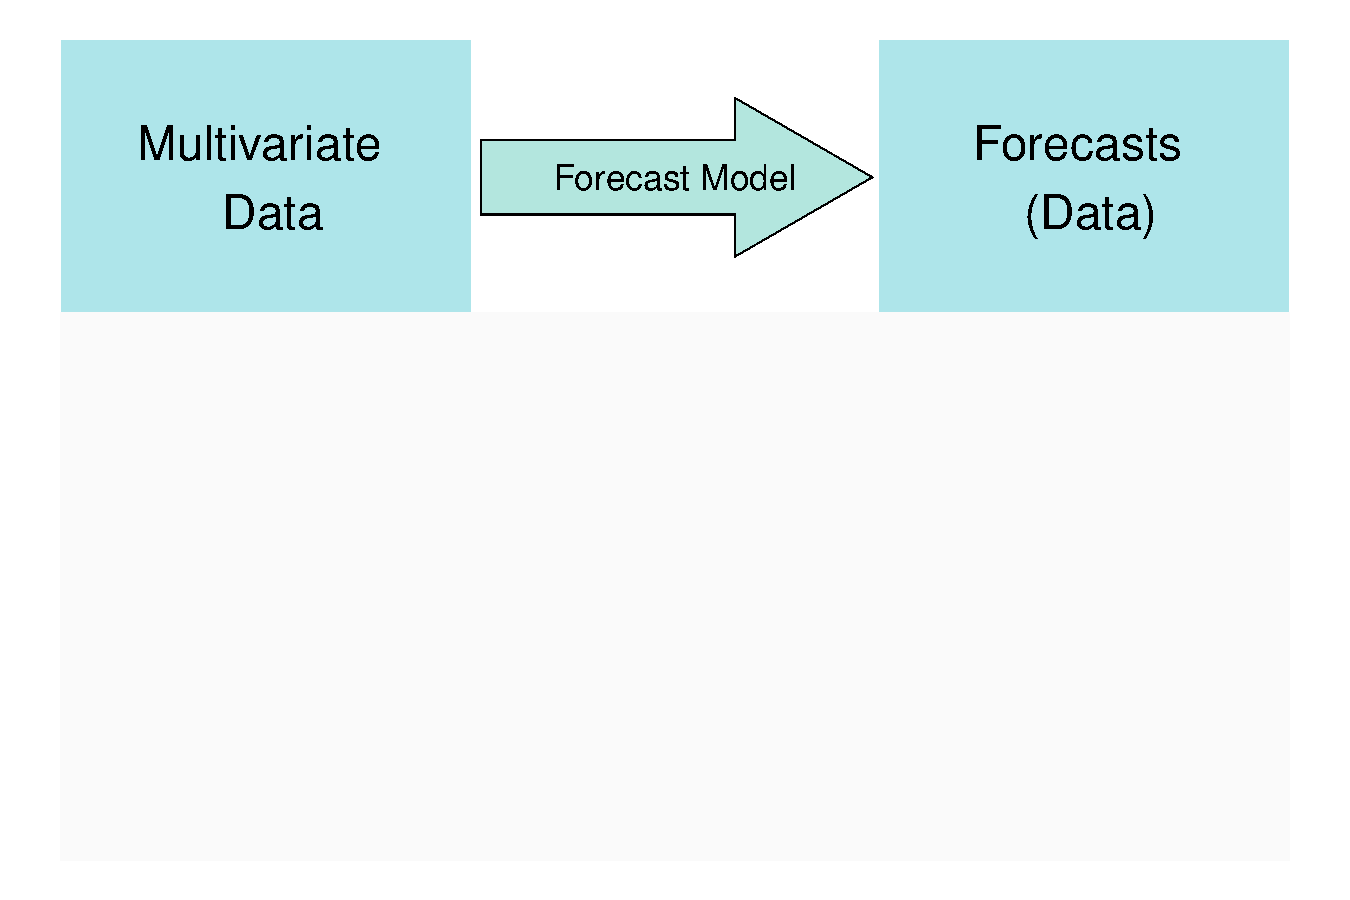
\includegraphics[width=\linewidth]{plot/p_others}
\end{frame}

\begin{frame}{What we do}
\protect\hypertarget{what-we-do}{}
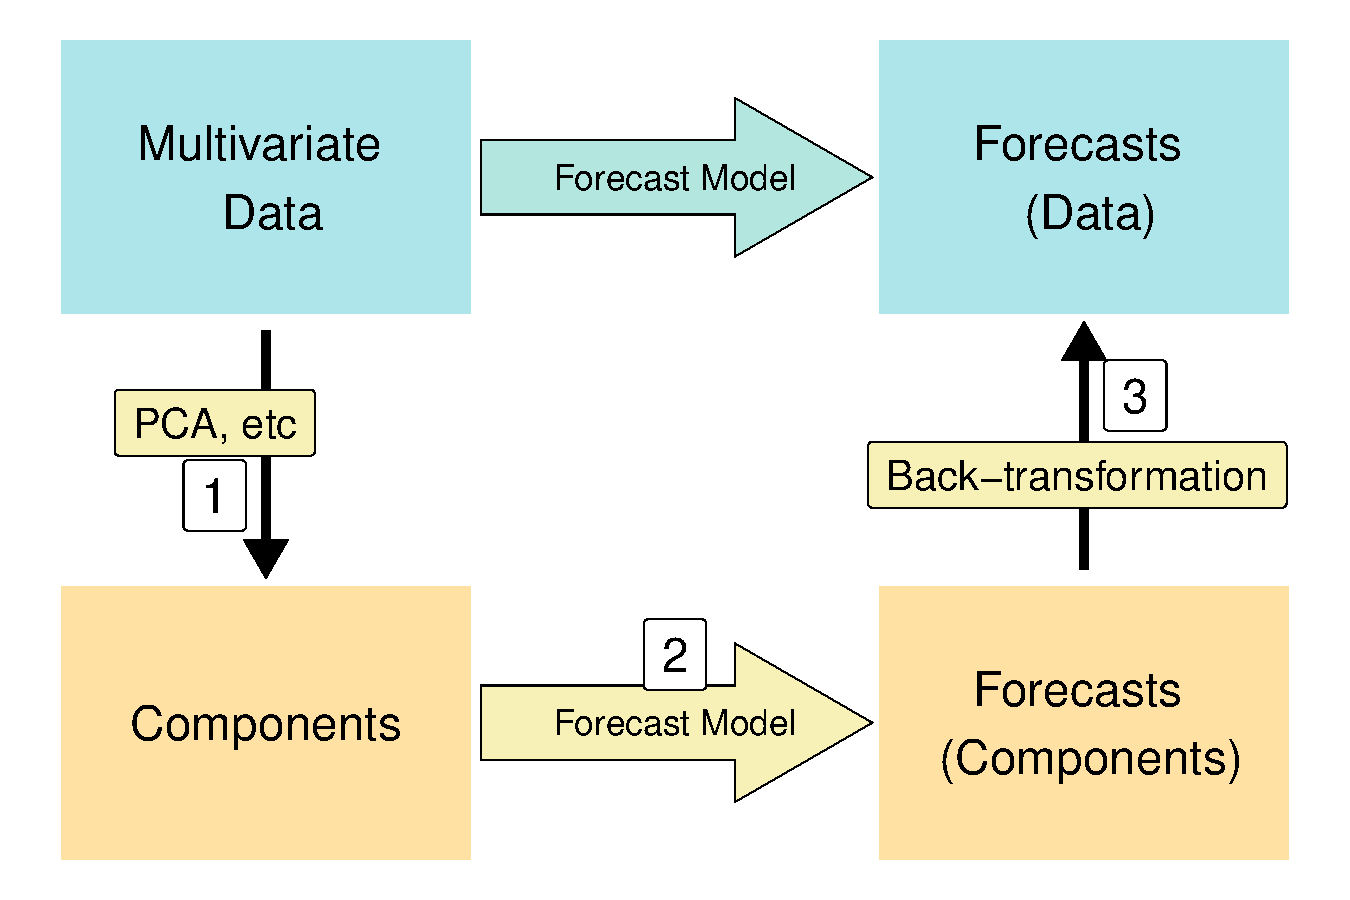
\includegraphics[width=\linewidth]{plot/p_ours}
\end{frame}

\begin{frame}{Australian tourism data}
\protect\hypertarget{australian-tourism-data}{}
\begin{itemize}
\tightlist
\item
  The data include tourism information on seven states and territories
  which can be divided into 77 regions

  \begin{itemize}
  \tightlist
  \item
    For example, Melbourne, Sydney, East Coast
  \end{itemize}
\end{itemize}

\begin{block}{Visitor nights}
\protect\hypertarget{visitor-nights}{}
The total number of nights spent by Australians away from home recorded
monthly
\end{block}
\end{frame}

\begin{frame}{Total and Region}
\protect\hypertarget{total-and-region}{}
\begin{center}
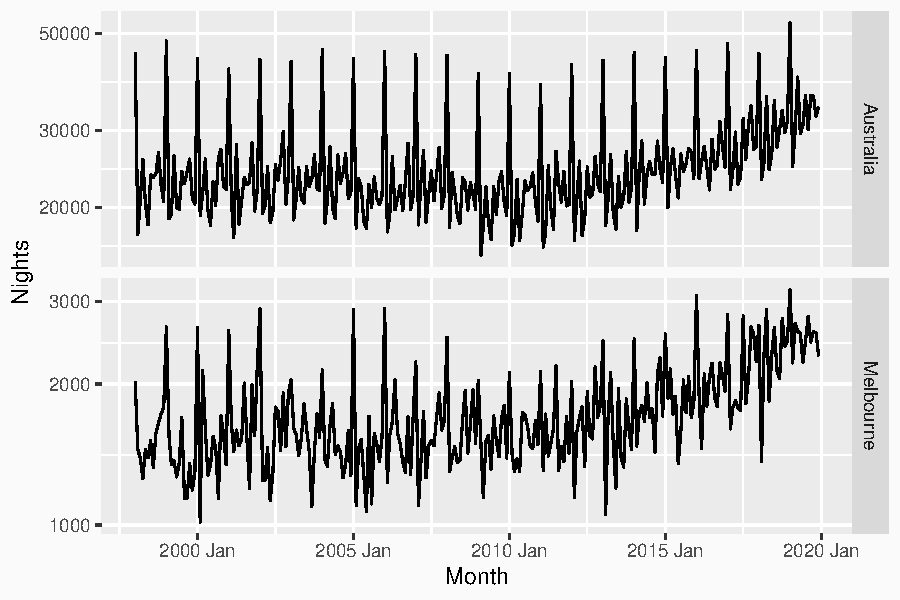
\includegraphics[width=\linewidth]{plot/p_aus_mel}
\end{center}
\end{frame}

\begin{frame}{Melbourne and Sydney}
\protect\hypertarget{melbourne-and-sydney}{}
\begin{center}
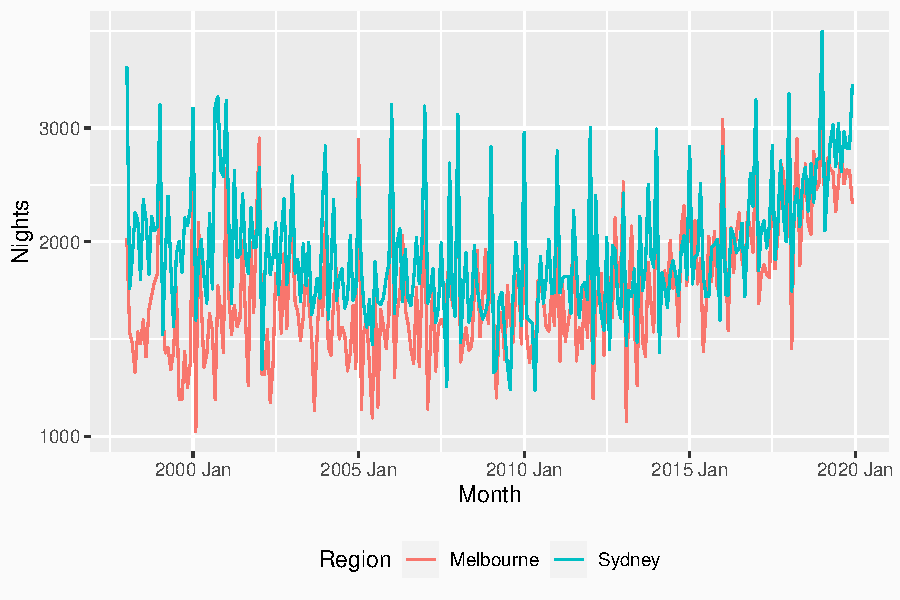
\includegraphics[width=\linewidth]{plot/p_syd_mel}
\end{center}
\end{frame}

\begin{frame}{Intuition}
\protect\hypertarget{intuition}{}
\begin{block}{Observation}

1. Better signal-noise ratio in the linear combination.

\pause
2. Similar patterns are shared by different series.
\end{block}

\pause

\begin{alertblock}{One step further}
Finding components that have better signal-noise ratio:


1. Easy to forecast;

2. Capturing the common signals;

3. Improving forecast of original series.
\end{alertblock}
\end{frame}

\begin{frame}{Literature}
\protect\hypertarget{literature}{}
\begin{block}{Factor model \citep{Bai2008-of}}
\protect\hypertarget{factor-model-bai2008-of}{}
\begin{enumerate}
\tightlist
\item
  Linear transformation
\item
  VAR models
\end{enumerate}
\end{block}

\begin{block}{Dynamic Factor Machine Learning
\citep[DFML,][]{DeStefani2021-nt}}
\protect\hypertarget{dynamic-factor-machine-learning-dfml-destefani2021-nt}{}
\begin{enumerate}
\tightlist
\item
  Nonlinear transformations with an inherent two-way mapping

  \begin{itemize}
  \tightlist
  \item
    Autoencoder
  \end{itemize}
\item
  Machine learning forecast methods
\end{enumerate}
\end{block}
\end{frame}

\begin{frame}{Our differences}
\protect\hypertarget{our-differences}{}
\begin{enumerate}
\tightlist
\item
  Allowing nonlinear transformations
\item
  Allowing transformations without an inverse function
\item
  Mappings between forecasts of the components and forecasts of the
  original series
\item
  Arbitrary forecast models
\end{enumerate}
\end{frame}

\begin{frame}{Overview}
\protect\hypertarget{overview}{}
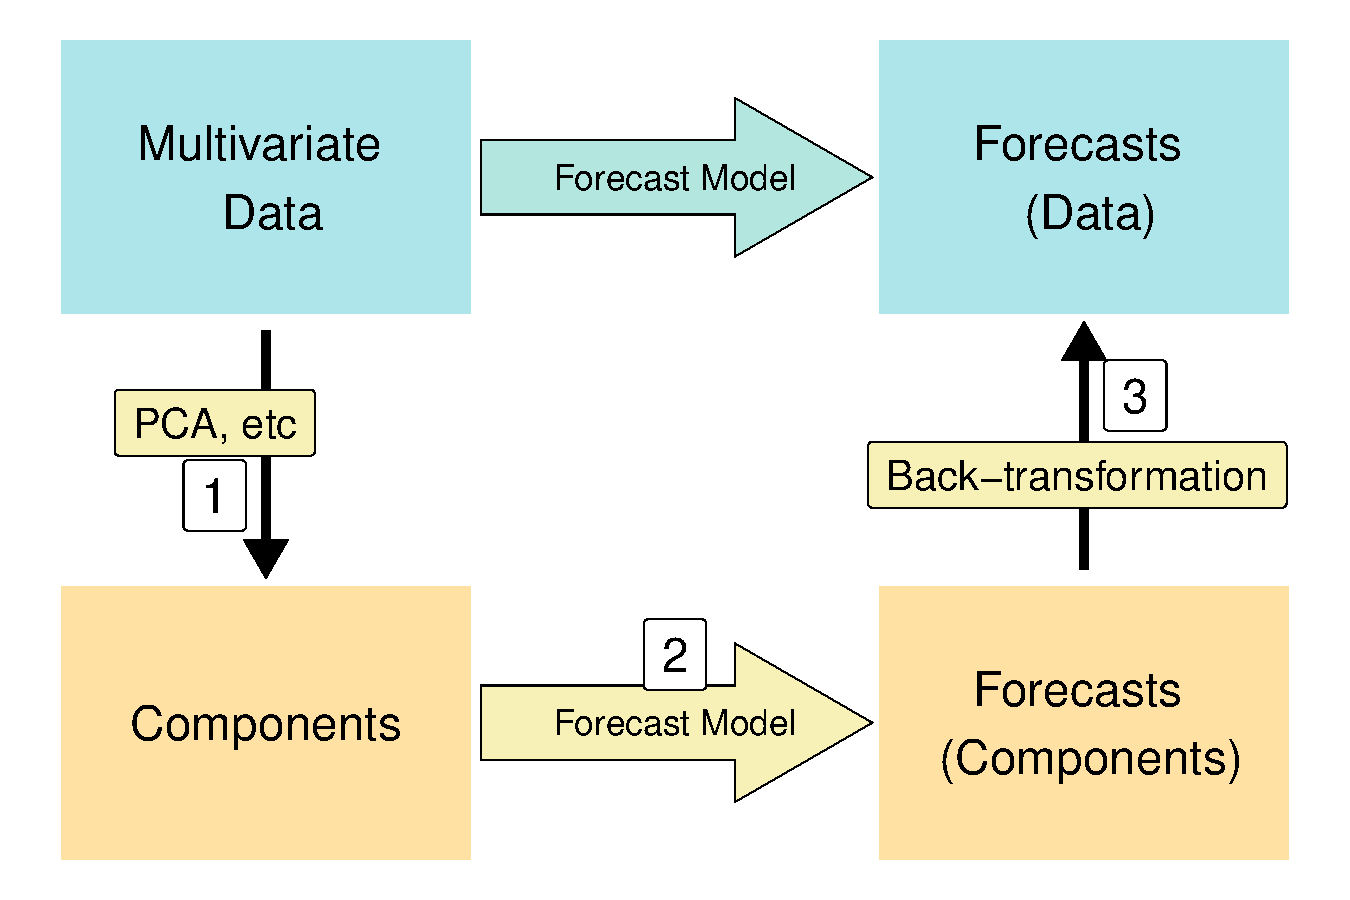
\includegraphics[width=\linewidth]{plot/p_ours}
\end{frame}

\begin{frame}{Overview}
\protect\hypertarget{overview-1}{}
\begin{center}
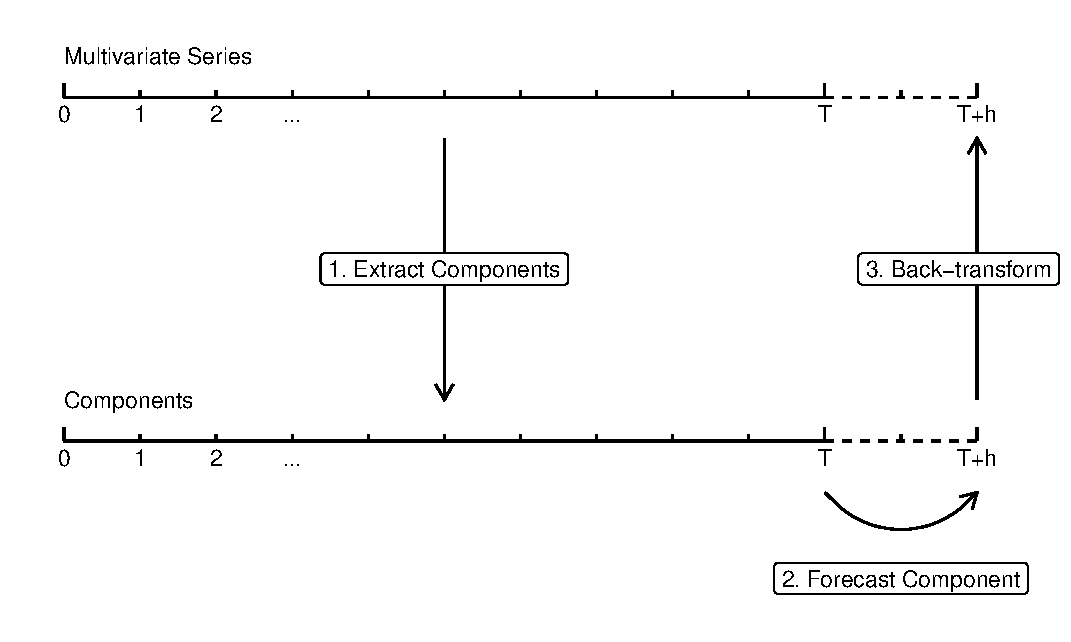
\includegraphics[width=\linewidth]{plot/p_timeline}
\end{center}
\end{frame}

\begin{frame}{1. Components: Linear}
\protect\hypertarget{components-linear}{}
Taking the first \(q\) linear combinations
\[\underset{T\times k}{\bm{Y}}\underset{k\times q}{\bm{W}}=\underset{T\times q}{\bm{C}},\]
where \(\bm{C}\) is the first \(q\) components, \(\bm{W}\) is the
weighting matrix.

\begin{block}{Principal Component Analysis (PCA)}
\protect\hypertarget{principal-component-analysis-pca}{}
Finding the weights matrix so that the resulting components
\alert{\textbf{maximise variance}}
\end{block}
\end{frame}

\begin{frame}
\begin{block}{Forecastable Component (ForeC)}
\protect\hypertarget{forecastable-component-forec}{}
Forecastable components \citep{Goerg2013-yu} maximise
\alert{forecastability}, finding linear combinations with
\alert{most regular patterns}

\centerline{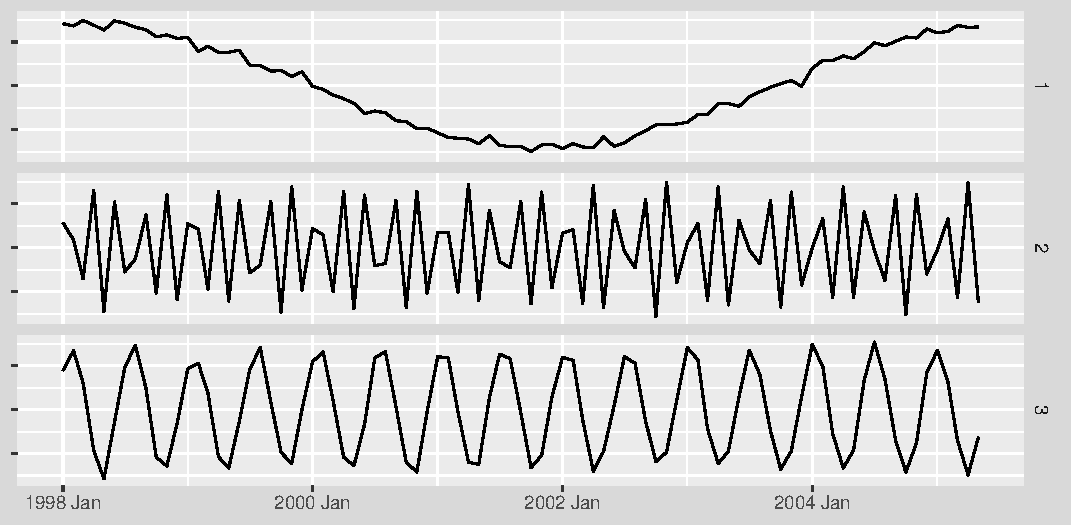
\includegraphics[width=\linewidth]{plot/p_forec}}
\end{block}
\end{frame}

\begin{frame}{1. Component: Nonlinear}
\protect\hypertarget{component-nonlinear}{}
\begin{block}{Manifold learning}
\protect\hypertarget{manifold-learning}{}
Nonlinear dimension reduction that preserves the distances between
points (relative locations of points) on a manifold

\begin{itemize}
\tightlist
\item
  Isomap, Laplacian Eigenmaps
\item
  No back-transformation methods available
\end{itemize}
\end{block}
\end{frame}

\begin{frame}{2. Forecast model}
\protect\hypertarget{forecast-model}{}
\begin{block}{Arbitrary choice of forecast models}
\protect\hypertarget{arbitrary-choice-of-forecast-models}{}
\begin{itemize}
\tightlist
\item
  ARIMA
\item
  Exponential smoothing
\item
  Dynamic regression models
\item
  Machine learning methods
\item
  etc
\end{itemize}
\end{block}
\end{frame}

\begin{frame}{3. Back-transformation}
\protect\hypertarget{back-transformation}{}
\begin{enumerate}
\tightlist
\item
  Construct a training set

  \begin{itemize}
  \tightlist
  \item
    Bootstrap to increase the sample size
  \item
    Expanding window to cover more sample values
  \item
    Redo Component Extraction and Component Forecast on each
    bootstrapped set
  \end{itemize}
\item
  Fit a back-transformation model using the above as the sample
\end{enumerate}
\end{frame}

\begin{frame}{Construct Training Set}
\protect\hypertarget{construct-training-set}{}
\begin{center}
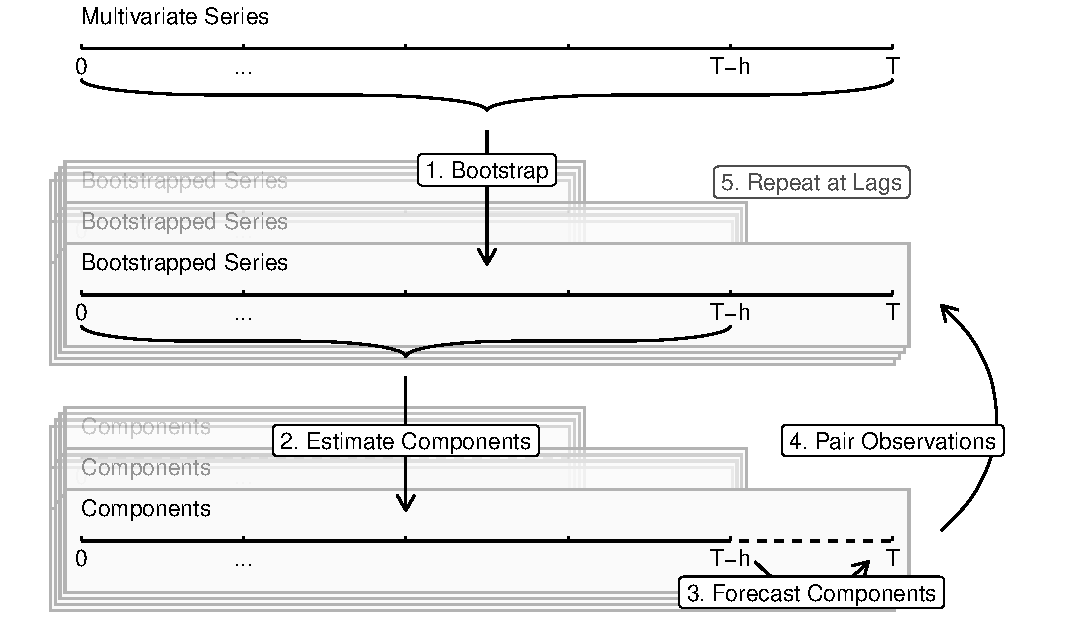
\includegraphics[width=\linewidth]{plot/p_backtransform}
\end{center}
\end{frame}

\begin{frame}{Bootstrap}
\protect\hypertarget{bootstrap}{}
\begin{block}{\citet{Bergmeir2016-yx}}
\protect\hypertarget{bergmeir2016-yx}{}
\begin{enumerate}
\tightlist
\item
  Box Cox Transformation

  \begin{itemize}
  \tightlist
  \item
    Stabilising variance
  \end{itemize}
\item
  Seasonal and Trend decomposition using Loess (STL)

  \begin{itemize}
  \tightlist
  \item
    Separating series into trend, seasonality and the stationary
    remainder
  \end{itemize}
\item
  Moving Block Bootstrap (MBB)

  \begin{itemize}
  \tightlist
  \item
    Bootstrapping stationary remainder
  \end{itemize}
\item
  Adding back trend and seasonality. Reversing Box Cox transformation.
\end{enumerate}
\end{block}
\end{frame}

\begin{frame}{STL Decomposition}
\protect\hypertarget{stl-decomposition}{}
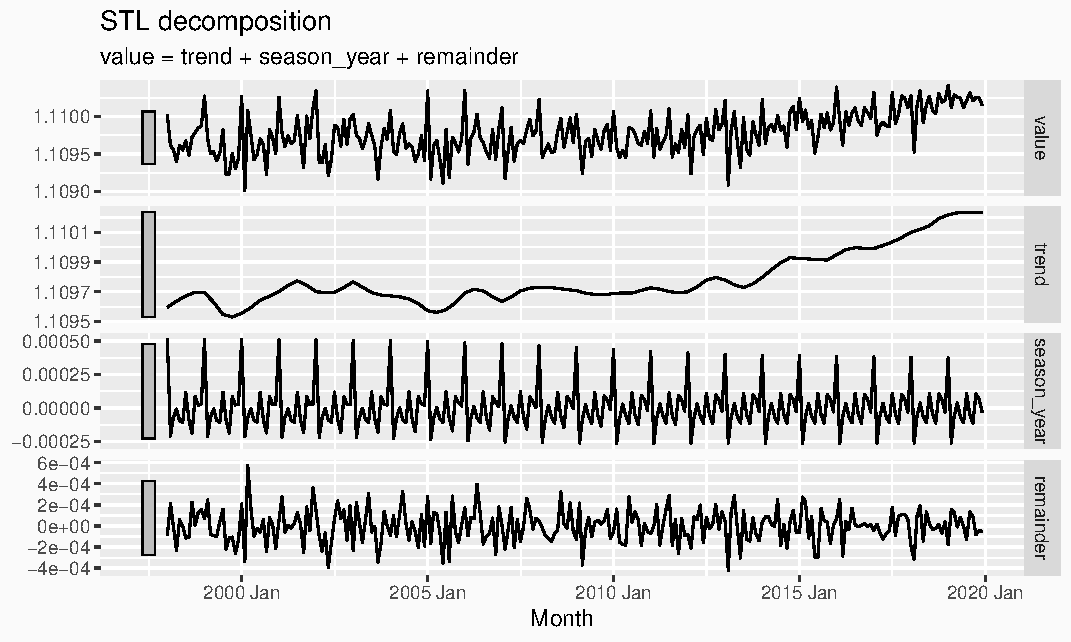
\includegraphics[width=\linewidth]{plot/p_stl}
\end{frame}

\begin{frame}{MMB on the remainder}
\protect\hypertarget{mmb-on-the-remainder}{}
\begin{center}
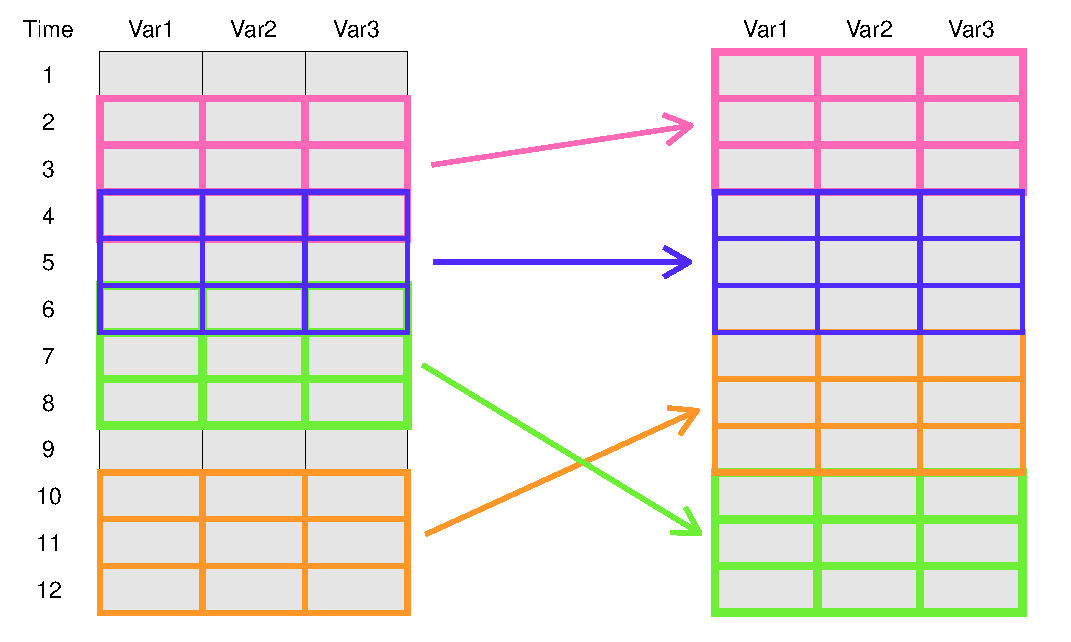
\includegraphics[width=\linewidth]{plot/p_mmb}
\end{center}
\end{frame}

\begin{frame}{Results}
\protect\hypertarget{results}{}
\begin{block}{Performance Measure (cross-validation)}
\protect\hypertarget{performance-measure-cross-validation}{}
\[
mRMSSE = \frac{1}{Mk}\sum^{M}_j\sum^{k}_i
\sqrt{\frac
{(y_{T-j+h,i}-\hat{y}_{T-j, h,i})^2}
{\frac{1}{T-j-\nu}\sum^{T-j}_{t={1+\nu}}(y_{ti} - y_{t-\nu, i})^2}}.
\]
\end{block}

\begin{block}{Multiple Comparisons with the Best (MCB)}
\protect\hypertarget{multiple-comparisons-with-the-best-mcb}{}
Compare Average ranks of mRMSSE in cross-validations
\citep{Koning2005-ch}
\end{block}

\begin{block}{Forecast model}
\protect\hypertarget{forecast-model-1}{}
Automatically selected ExponenTial Smoothing (ETS) model using AICc
\end{block}
\end{frame}

\begin{frame}{Australian tourism}
\protect\hypertarget{australian-tourism}{}
\begin{figure}

{\centering \includegraphics{components-forecast_files/figure-beamer/unnamed-chunk-10-1.pdf}

}

\end{figure}
\end{frame}

\begin{frame}{Outcome}
\protect\hypertarget{outcome}{}
\begin{itemize}
\item
  Generic method to forecast using lower dimensional components with
  arbitrary choices of components and forecast models
\item
  Robust to the number of components
\item
  PCA and ISOMAP are most competitive
\item
  Random forest works best for longer term forecast. Linear models work
  best for short term forecast.
\end{itemize}
\end{frame}

\hypertarget{appendix}{%
\section{Appendix}\label{appendix}}

\begin{frame}{Isomap}
\protect\hypertarget{isomap}{}
\begin{enumerate}
\tightlist
\item
  Construct Nearest Neighbour Graph
\item
  Estimate the Geodesic distances (distances along a manifold)
\item
  Apply Classical MDS

  \begin{itemize}
  \tightlist
  \item
    Input distances
  \item
    Output coordinates in a lower dimension with similar distances
  \end{itemize}
\end{enumerate}

\begin{block}{Other Components}
\protect\hypertarget{other-components}{}
Laplacian Eigenmaps, etc
\end{block}
\end{frame}

\begin{frame}{Isomap}
\protect\hypertarget{isomap-1}{}
\begin{center}
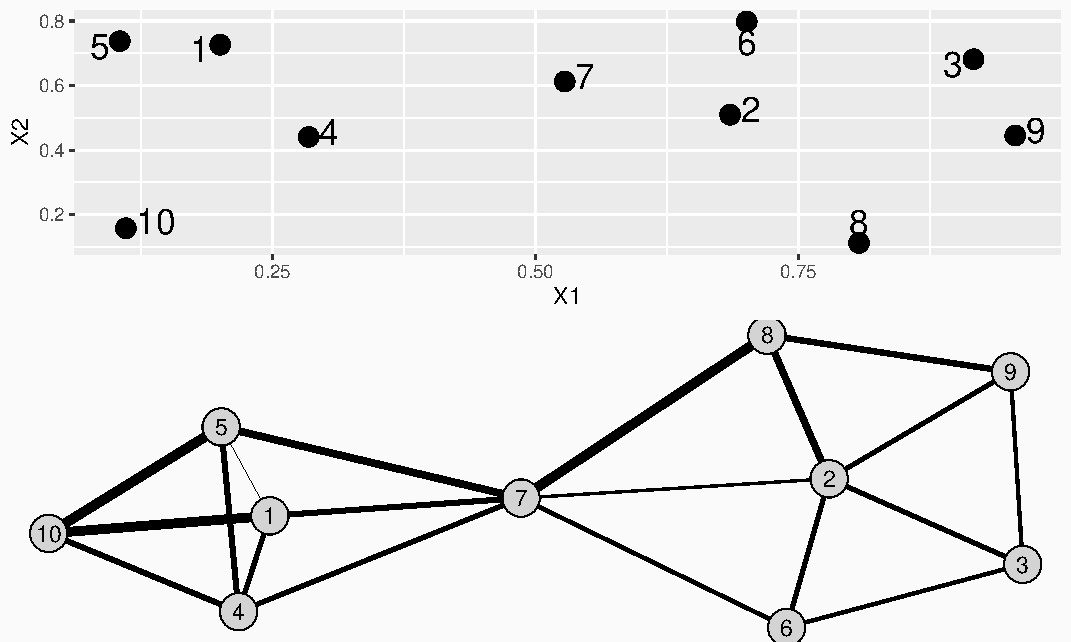
\includegraphics[width=\linewidth]{plot/p_isomap1}
\end{center}
\end{frame}

\begin{frame}{Isomap}
\protect\hypertarget{isomap-2}{}
\begin{center}
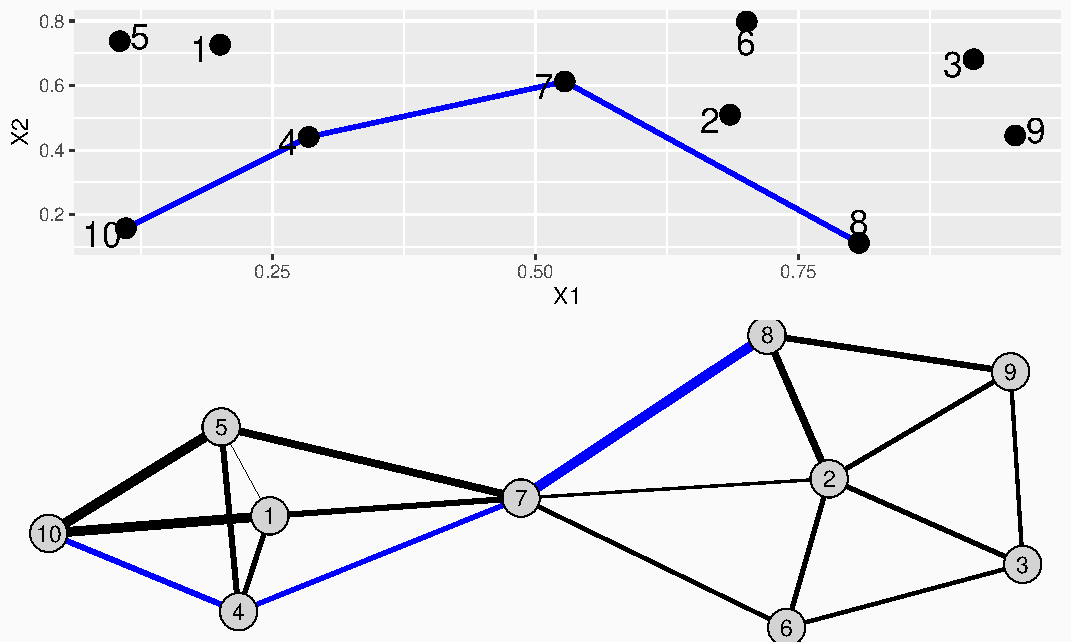
\includegraphics[width=\linewidth]{plot/p_isomap2}
\end{center}
\end{frame}

\begin{frame}{Components Clustering}
\protect\hypertarget{components-clustering}{}
\begin{block}{Problem}
\protect\hypertarget{problem}{}
\begin{itemize}
\tightlist
\item
  Some components do not have order.

  \begin{itemize}
  \tightlist
  \item
    e.g.~ForeCA
  \end{itemize}
\item
  Components from the bootstraps should provide similar information
  about the future
\end{itemize}
\end{block}
\end{frame}

\begin{frame}{Components Clustering: Before}
\protect\hypertarget{components-clustering-before}{}
\begin{center}
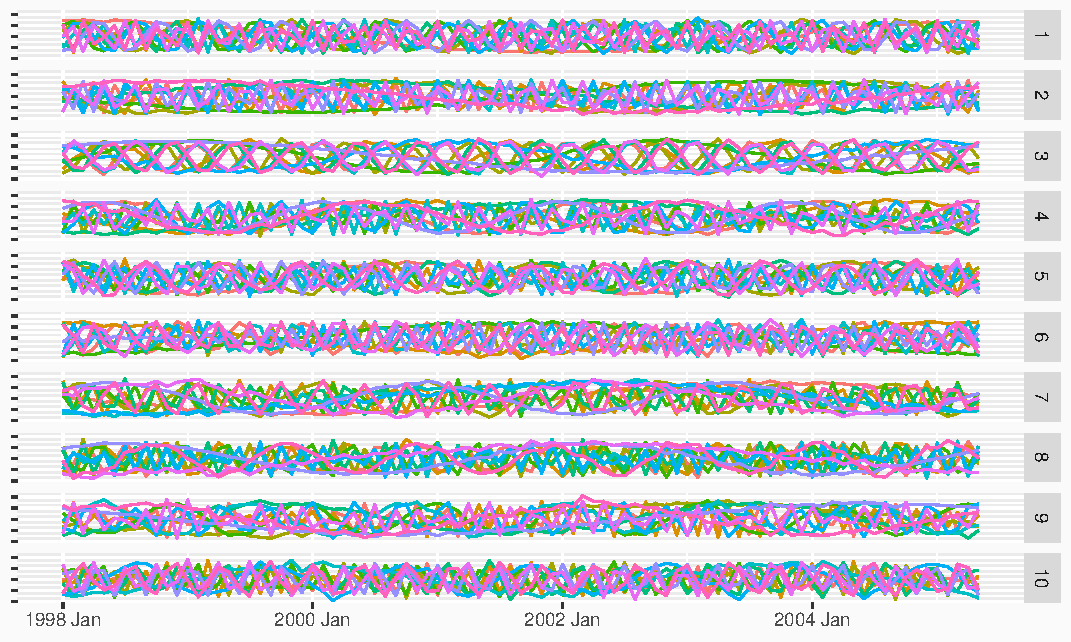
\includegraphics[width=\linewidth]{plot/p_cluster_before}
\end{center}
\end{frame}

\begin{frame}{Components Clustering}
\protect\hypertarget{components-clustering-1}{}
\begin{block}{Solution: Feature-based clustering}
\protect\hypertarget{solution-feature-based-clustering}{}
\begin{enumerate}
\tightlist
\item
  Calculate features from each component

  \begin{itemize}
  \tightlist
  \item
    Highly comparative time-series analysis: \citet{Fulcher2017-zl}
  \item
    \citet{Talagala2023-yi}
  \end{itemize}
\item
  Cluster the features

  \begin{itemize}
  \tightlist
  \item
    K-means with cannot-link constraints: COP kmeans
    \citet{Wagstaff2001-vc}
  \end{itemize}
\end{enumerate}
\end{block}
\end{frame}

\begin{frame}{Components Clustering: After}
\protect\hypertarget{components-clustering-after}{}
\begin{center}
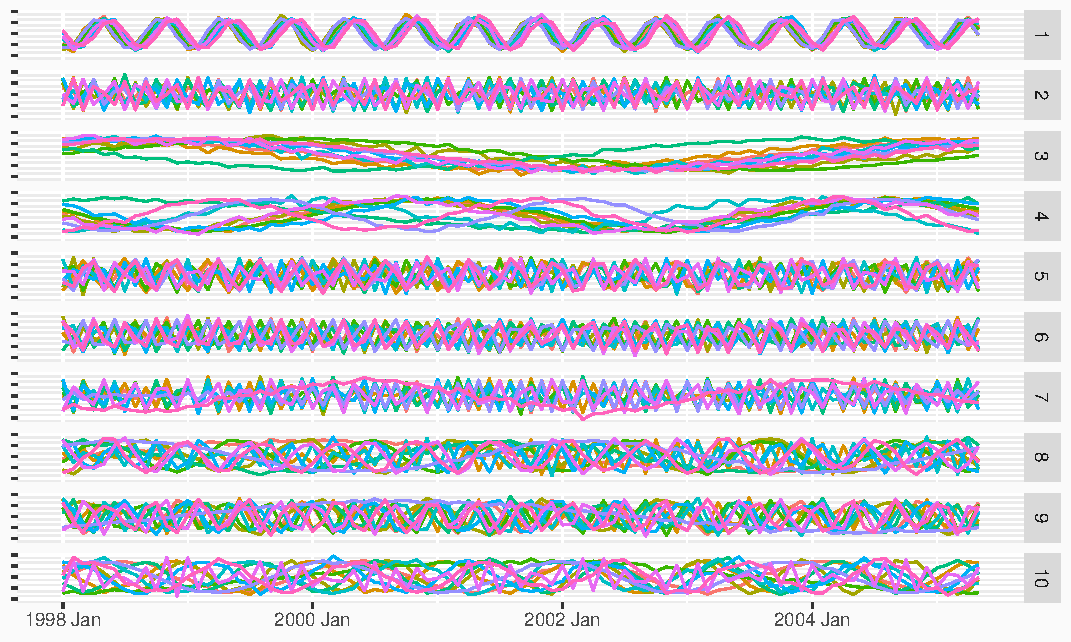
\includegraphics[width=\linewidth]{plot/p_cluster_after}
\end{center}
\end{frame}

\begin{frame}{Overview}
\protect\hypertarget{overview-2}{}
\centerline{
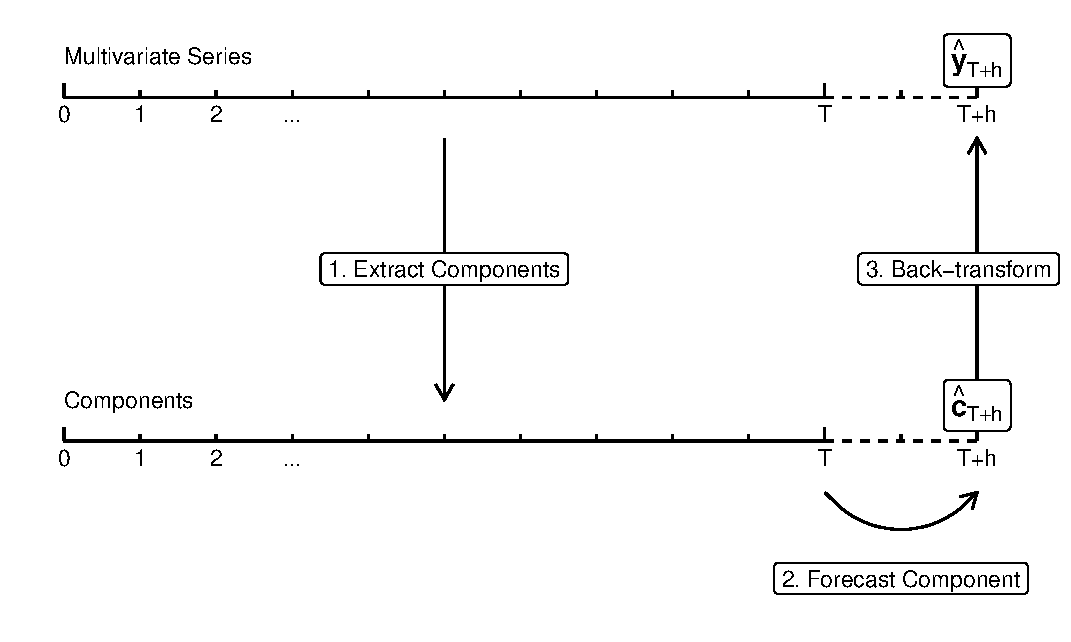
\includegraphics[width=\linewidth]{plot/p_timeline_notation}
}
\end{frame}

\begin{frame}{Construct Training Set}
\protect\hypertarget{construct-training-set-1}{}
\begin{center}
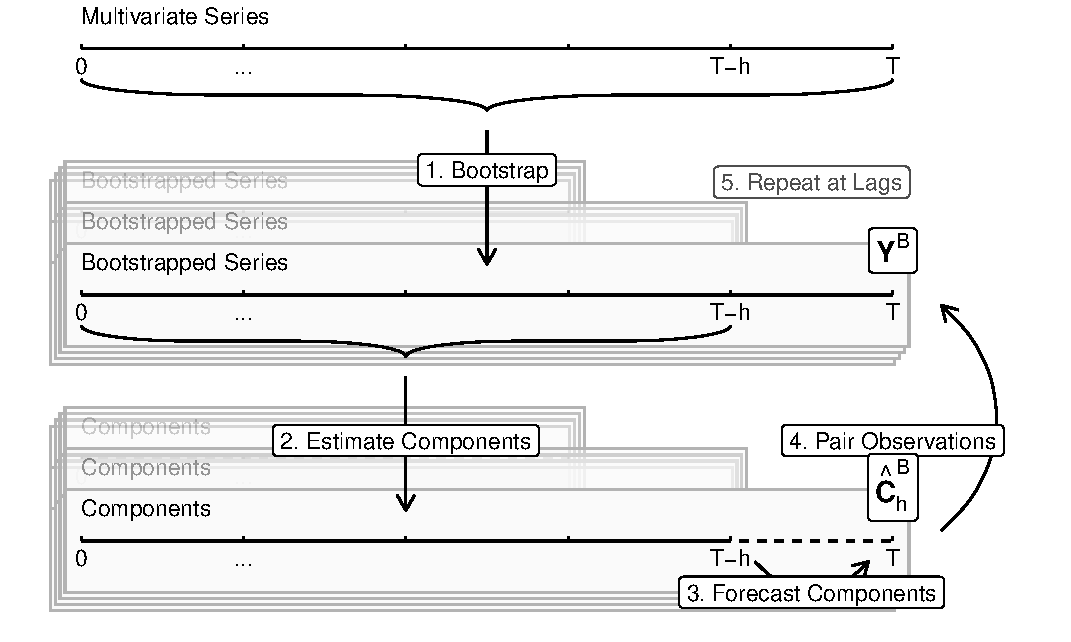
\includegraphics[width=\linewidth]{plot/p_backtransform_notation}
\end{center}
\end{frame}

\begin{frame}{Back-transformation Model}
\protect\hypertarget{back-transformation-model}{}
\begin{itemize}
\tightlist
\item
  \(\hat{\bm{C}}^\mathsf{B}_h\): \(h\)-step-ahead forecasts of
  components from different bootstraps at different lags
\item
  \(\bm{Y}^\mathsf{B}\): the corresponding ``real'' values of the
  original series from bootstraps
\item
  \(\hat{\bm{c}}_{T+h}\): \(h\)-step-ahead forecasts of components of
  the original series
\item
  \(\hat{\bm{y}}_{T+h}\): \(h\)-step-ahead forecasts of the original
  series
\item
  \(\bm{S}\): collection of seasonal dummies corresponding to
  \(\hat{\bm{C}}^\mathsf{B}_h\)
\item
  \(\bm{s}_{T+h}\): seasonal dummies at time \(T+h\)
\item
  \(\bm{X} = \begin{bmatrix}\hat{\bm{C}}^\mathsf{B}_h & \bm{S}\end{bmatrix}\)
\end{itemize}
\end{frame}

\begin{frame}{Back-transformation Model}
\protect\hypertarget{back-transformation-model-1}{}
\[
\hat{\bm{y}}_{T+h} = 
f(\hat{\bm{c}}_{T + h}, \bm{s}_{T+h})
\]

\begin{block}{Discounted Least Squares (DLS)}
\protect\hypertarget{discounted-least-squares-dls}{}
\[
\hat{\bm{y}}_{T+h} = 
\hat{\bm{B}}'
\begin{bmatrix}
\hat{\bm{c}}_{T + h} \\ \bm{s}_{T+h}
\end{bmatrix}
\]

\[
\hat{\bm{B}} = (\bm{X}'\bm{U}\bm{X})^{-1}\bm{X}'\bm{U}\bm{Y}^\mathsf{B}, 
\]
\end{block}
\end{frame}

\begin{frame}{Discounted Least Squares (DLS)}
\protect\hypertarget{discounted-least-squares-dls-1}{}
\[
u = \delta(1-\delta)^{\text{YearLag}}
\]

\begin{center}
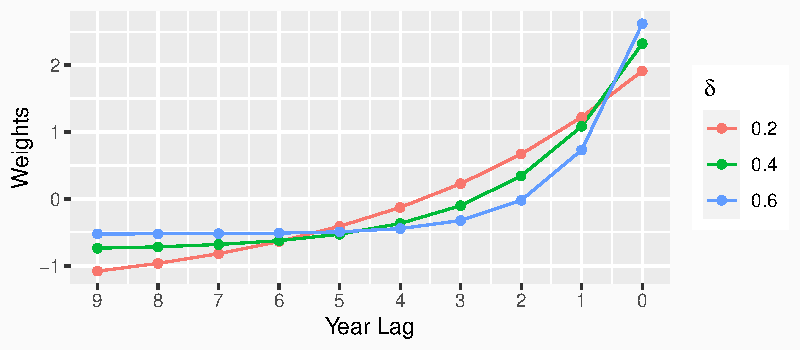
\includegraphics[width=\linewidth]{plot/p_dls}
\end{center}
\end{frame}

\begin{frame}{Australian tourism: PCA}
\protect\hypertarget{australian-tourism-pca}{}
\begin{figure}

{\centering \includegraphics[width=1\textwidth,height=1\textheight]{components-forecast_files/figure-beamer/unnamed-chunk-18-1.pdf}

}

\end{figure}
\end{frame}

\begin{frame}{Box Cox Transformation}
\protect\hypertarget{box-cox-transformation}{}
\begin{block}{Modified version of \citet{Bickel1981-hv}}
\protect\hypertarget{modified-version-of-bickel1981-hv}{}
\[
w_t  =
\begin{cases}
\log(y_t) & \text{if } \lambda=0;  \\
(\text{sign}(y_t)|y_t|^\lambda-1)/\lambda & \text{otherwise},
\end{cases}
\]
\end{block}

\begin{block}{Reverse transformation}
\protect\hypertarget{reverse-transformation}{}
\[
y_{t} =
\begin{cases}
\exp(w_{t}) & \text{if } \lambda=0;\\
\text{sign}(\lambda w_t+1)|\lambda w_t+1|^{1/\lambda} & \text{otherwise}.
\end{cases}
\]
\end{block}
\end{frame}

\begin{frame}{Box Cox Transformation}
\protect\hypertarget{box-cox-transformation-1}{}
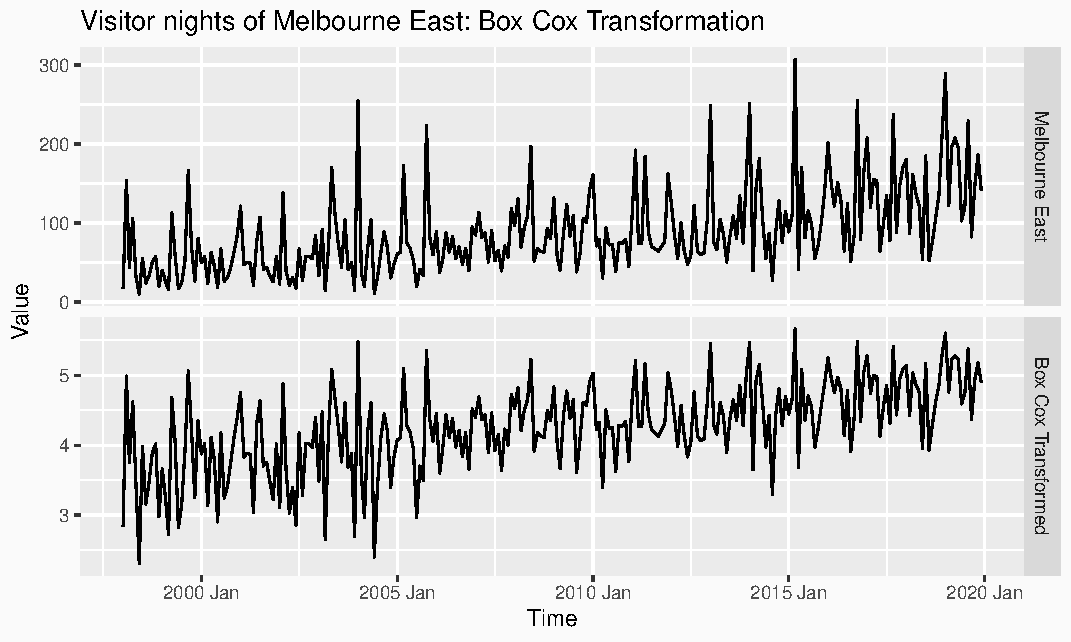
\includegraphics[width=\linewidth]{plot/p_boxcox}
\end{frame}

                    \renewcommand\refname{References}
              \begin{frame}[allowframebreaks]{References}
    \fontsize{9}{10}\selectfont
    \bibliographytrue
    \bibliography{refs.bib}
    \end{frame}
  


\end{document}
